\documentclass{NIHGrant}
\author{Andrew Sugarman}
\date{\today}
\title{High-Resolution Wide-Field 3D Histopathology for the Morphological Characterization of Prostate Cancer}
\newcommand{\Id}[2]{\text{Id}_{#1}(#2)} % Identification Region
\let\inf\rest \DeclareMathOperator*{\inf}{Inf} % Infimum, note: * undersets limits
\newcommand{\E}{\mathbb{E}} % Nice Infimum
\newcommand{\set}[1]{\mathbf{#1}} % Notation for Sets
\newcommand{\proc}[1]{\mathcal{#1}} % Notation for Stochastic Process
\newcommand{\proca}[2]{\proc{#1}(#2)} % Notation for \proc evaluated at
\newcommand{\procaa}[3]{[\proc{#1}(#2)]_{#3}} % Notation for element of \proca vector
\newcommand{\R}{\mathbb{R}} % Real Space
\renewcommand{\S}{\mathbb{S}} % Simplex
\newcommand{\Z}{\mathbb{Z}} % Integers


\newcommand{\citetram}{\cite{nixon2022statistical}}


% \newtheorem{theorem}{Theorem}
\newtheorem{definition}{Definition}
\newtheorem{corollary}{Corollary}
\newtheorem{lemma}{Lemma}
\newtheorem{proposition}{Proposition}

\newtheoremstyle{theorem}% name
{\topsep}% space above
{\topsep}% space below
{}% body font
{}% indent amount
{\itshape}% theorem head font
{}% punctuation after theorem head
{.5em}% space after theorem head
{\scshape{\thmname{#1}}\thmnumber{ #2}\thmnote{ (#3)}.~---}% theorem head spec
\theoremstyle{theorem}
\newtheorem{theorem}{Theorem}

\usepackage{microtype}

\begin{document}
\maketitle
\newpage
\part*{Specific Aims}

Abnormal tissue morphology is a hallmark of many soft tissue tumors. Characterization of morphology at the macroscopic or microscopic level can provide insights critical to diagnosis, prognosis, therapeutic design, and even basic research. At the macroscopic level, a variety of three-dimensional (3D) imaging technologies (e.g., MRI, CT, and PET-CT) exist and allow clinicians to stage cancer and direct therapies based on the size and shape of lesions~\cite{primakov_automated_2022,katiyar_quantification_2023}. Complementing these imaging technologies, machine learning and statistics advances allow researchers to quantify morphologic characteristics to aid cancer diagnosis and prognosis~\cite{lawson_persistent_2019,crawford_predicting_2020}.
Morphology is just as critical at the microscopic level. For example, in prostate cancer, glandular morphology is paramount to cancer staging and is the main component of the popular Gleason score~\cite{gordetsky_grading_2016,epstein_prostate_2018}. However, at the microscopic level, clinicians and researchers have been limited primarily to qualitative assessment of two-dimensional, slide-based imaging~\cite{liu_harnessing_2021}. Assessing morphology in only two dimensions can be sub-optimal~\cite{ozkan_interobserver_2016,xie_prostate_2022,koyuncu_visual_2023}. For example, the angle at which a two-dimensional tissue slice is taken can alter conclusions about glandular morphology~\cite{serafin_nondestructive_2023} and is hypothesized to lead to the large variability in prostate cancer grading between observers~\cite{serafin_nondestructive_2023,flach_significant_2021}. In short, \emph{there is a paucity of tools available for assessing 3D tissue morphology at the microscopic level.}

Recent micro Computed Tomography (micro-CT) advances can facilitate high-resolution 3D imaging of biological tissue~\cite{albers_x-ray-based_2018,katsamenis_x-ray_2019}. In particular, synchrotron micro-CT techniques have demonstrated the ability to resolve cellular structures. However, these methods often require dedicated beamlines or are limited in their field of view~\cite{topperwien_contrast_2019,pinkert-leetsch_three-dimensional_2023,frost_3d_2023}. To address this problem, Dr.~Cheng's lab has shown how a novel wide-field detector can generate almost centimeter scale images at sub-micrometer resolution~\cite{yakovlev_wide-field_2022}. \uline{Recently, we developed a Propagation-Based phase-contrast CT (PBCT) imaging protocol that eliminates the need to stain tissue blocks and thereby permits direct imaging of clinical biopsies, which are often paraffin-embedded and challenging to stain.} Using this technology, we have been able to produce 3D images of prostate cancer and melanoma with the highest resolution to field of view ratio to date. In what follows, \uline{We propose to expand upon this technology and demonstrate its ability as both a clinical and research tool.} In Aim 1, we will optimize the PBCT protocol to ease future technology adoption. In Aims 2 and 3, we will evaluate the capabilities of this imaging technology as a clinical and research tool for prostate cancer.

\noindent
\paragraph*{Aim 1: Optimize PBCT imaging of Formalin-Fixed Paraffin-Embedded (FFPE) soft-tissue biopsies.}
Our preliminary results already establish that PBCT is capable of producing high-resolution images of soft-tissue biopsies even in settings where contrast-enhancing staining of tissue blocks is not possible. To optimize this protocol, we will develop a multi-tissue atlas demonstrating how key protocol parameters (e.g., x-ray energy and propagation distance) affect image characteristics including resolution and contrast in different tissue types such as mouse breast cancer, human oropharyngeal cancer, and human prostate cancer. This atlas will assist researchers in determining optimal imaging parameters for their studies.

\paragraph*{Aim 2: Evaluate utility of PBCT imaging for the grading of prostate cancer.}
We will collect the first micro-CT dataset of prostate cancer. Biopsies from disease subjects and age-matched healthy controls will be used to
assess and test the hypothesis that PBCT grading is non-inferior to standard slide-based imaging. Beyond this pilot study, these data will be made available publicly as a resource for the community.

\paragraph*{Aim 3: Quantify the morphological heterogeneity in prostate glands using computational persistent homology.}

Computational topology provides a rich suite of tools for quantifying 3D shapes in such a way that morphology can be included as covariates in statistical and machine learning-based cancer prognostics~\cite{primakov_automated_2022,crawford_predicting_2020}. In collaboration with Dr. Silverman, we will identify which topological summary statistics can best capture the morphologic differences between cancerous and healthy prostate glands. Using these statistics, we will then provide the first quantification of how glandular morphology varies spatially within a biopsy as a function of age and disease status. This quantification will provide novel biological insights into tumor heterogeneity and will inform the design of future studies of prostate cancer.  \\[5pt]
%
\noindent
%%%% my retry
Completing these aims will provide three critical outcomes: (1) the first micro-CT imaging protocol for the high-resolution 3D imaging of whole tissue blocks, (2) a clinical evaluation of this technology in the context of prostate cancer grading, and (3) the first quantitative study of morphological variation in prostate cancer. Finally, this research will provide me with the skills and expertise to pursue my long-term career goal of leading an independent research program in Oncology.

\newpage
\part*{Research Strategy}
\section*{Significance}
Abnormal morphology is a hallmark of many cancers and is critical in
diagnostic, prognostic, and treatment decisions~\cite{kumar_robbins_2017}. Both macroscopic
morphology (e.g., the shape of a tumor as a whole) and microscopic morphology
(e.g., the shape of prostate glands) are clinically important. While
clinicians and researchers have numerous tools available for assessing and
quantifying morphology at the macroscopic level, comparable tools are often
unavailable at the microscopic level. At the macroscopic level, clinicians
assess morphology using 3D imaging technologies such as magnetic resonance
imaging (MRI) or computed tomography (CT). Yet at the microscopic level,
morphological assessment is almost exclusively done by traditional 2D
slide-based imaging. Numerous studies have found that 2D imaging techniques can be
sub-optimal for assessing cancer morphology~\cite{xie_prostate_2022,koyuncu_visual_2023,pinkert-leetsch_three-dimensional_2023}. For example, in staging
prostate cancer, Koyuncu et al.~(2023)~\cite{koyuncu_visual_2023}
found that the slice angle used to prepare 2D
slides could alter the apparent morphology of glands and alter grading
decisions. It is hypothesized that such problems may be partially
responsible for the large variability in grading between individuals~\cite{ozkan_interobserver_2016}.
Outside of the imaging technologies themselves, the ubiquity of 3D images of
cancer have led to numerous statistical and machine learning advances that may
ultimate improve clinical care. For example, Crawford et al.~(2020)~\cite{crawford_predicting_2020} showed that
computational topology could be used identify the morphological biomarkers for
MRI imaging of Glioblastoma that were more predictive of patient outcomes than
traditional clinical metrics or molecular biomarkers. Tools such
as those developed by Crawford et al.~\cite{crawford_predicting_2020,lawson_persistent_2019} cannot be applied at the
microscopic level due to the lack of 3D imaging data. In short,
\emph{assessment of cancer morphology is limited at the microscopic level due
  to a lack of available imaging technologies}.

% rewrite this paragraph with emphasis on sample prep and
Several approaches to 3D microscopic imaging have recently been proposed.
These include the hybrid Open-Top Light-Sheet microscopy (OTLS) illustrated in
Glaser et al.~(2022)~\cite{glaser_hybrid_2022} and a number of related methods collectively called
micro-CT~\cite{katsamenis_x-ray_2019,topperwien_contrast_2019,frost_3d_2023,cheng_whole-animal_2011,ding_computational_2019}. OTLS is a 3D imaging method that relies on tissue clearing and fluorescent staining of tissue samples. OTLS permits high-quality
volumetric imaging of whole biopsies without requiring repeated sectioning.
Yet, OTLS requires complicated sample preparation procedures involving tissue clearing and staining with fluorescent markers. Micro-CT however can provide 3D imaging of biological samples at 0.5$\mu$m isotropic voxel resolution, doing so \uline{without the use of tissue clearing or the addition of any fluorescent markers}~\cite{pinkert-leetsch_three-dimensional_2023,yakovlev_wide-field_2022,ding_computational_2019,topperwien_correlative_2020}.
% Moreover two recent developments have greatly enhanced the
% applicability of micro-CT by expanding the field-of-view and removing the
% dependence on contrast-enhancing staining.
% outtake: In contrast, micro-CT stands out as an
% alternative to OTLS which can obtain substantially higher resolution~[CITE].

While multiple groups have shown that micro-CT is capable of producing
high-resolution cellular and sub-cellular imaging, these technologies have
been limited by their narrow field-of-view. For example, while Pinkert-Leetsch et al.
demonstrated they could resolve nuclei within pancreatic adenocarcinoma, their entire field of view was limited to 1.6 by 1.4mm~\cite{pinkert-leetsch_three-dimensional_2023}. This field-of-view is much smaller than most biopsy specimens, requiring the user to acquire many scans to cover just one sample. The Cheng Lab
recently addressed this issue and demonstrated that a novel wide-field
detector allowed for nearly centimeter scale (whole-biopsy) imaging at sub-micrometer (0.5$\mu$m) isotropic voxel
resolution~\cite{yakovlev_wide-field_2022}.
%%% Perhaps include the explicit field of view of max's detector 5x4mm
%%% include burden of stitiching?

Contrast-enhancing stains are typically required to obtain high-quality
micro-CT images of biological tissue~\cite{ding_computational_2019,katz_whole-organism_2021,busse_three-dimensional_2018,metscher_microct_2009}. Yet many clinical samples are
Formalin-Fixed and Paraffin-Embedded (FFPE) and do not take up those stains
without significant alterations to the sample such as deparaffinization. Recently, Frohn et al.~(2020)~\cite{frohn_3d_2020}, demonstrated that high-resolution stain-free
micro-CT of FFPE pancreatic biopsies could be obtained using Propagation-Based
phase-contrast CT and phase-retrieval algorithms developed for traditional
(macroscopic) CT~\cite{mohan_non-linear_2023}. In brief, PBCT reconstructs high-resolution 3D images
by using the fact that the phase of photons change differently depending on
their incident energy and the type of material they pass through. This is in contrast to traditional CT
imaging that primarily focuses on the magnitude of attenuation as photons pass through
a material~\cite{katz_whole-organism_2021,metscher_microct_2009}. However, two factors limit the utility of their approach. First,
they had the same limited field-of-view typical of micro-CT. Second, their
approach utilized a number of non-standard tools as part of the imaging apparatus
including Kirkpatrick-Baez (KB) mirrors and a waveguide, or an interferometer~\cite{frost_3d_2023,polikarpov_towards_2023,riedel_comparing_2023}.
% mention talbot interferometer
% clarify attenuation or avoid that distinction?
%%% is a reviewer going to ask why i am not just staining samples ahead of paraffinization?

Recently we have demonstrated that our wide-field detector could be combined with a modified PBCT protocol to obtain high-resolution,
whole-biopsy, stain-free micro-CT images of clinical biopsies (Figure 1).
Notably, our modified PBCT protocols do not requires KB mirrors or
waveguides and are therefore simpler than some of the prior PBCT protocols with
no appreciable decrease in resolution. With this development effective 3D
microscopic imaging of clinical biopsies is possible. In what follows, we propose
to expand upon this prior work. In Aim 1, we propose to optimize our modified
PBCT protocol and provide a multi-tissue atlas that researchers can use
determine optimal imaging parameter for different tissue types. Aims 2 and 3
then focus on the application of this technology to imaging prostate biopsies.
Aim 2 evaluates the utility of this technology in clinical settings while Aim 3
focuses on adapting quantitative tools developed for macroscopic morphometrics
to the microscopic domain. Beyond demonstrating the technology, Aims 2 and 3
provide novel insights into prostate cancer. For example, Aim 3 will provide the
first quantitative study of how the morphological features distinguishing
healthy versus cancerous prostate glands varies spatially within a tumor,
between individuals, as a function of age, and as a function of disease status.
Among other uses, that analysis can directly inform the design of future studies
of prostate cancer as it will directly inform estimates of effect sizes and
sampling variability.%reread to try and limit repetitiveness

\section*{Innovation}
% Dr. silverman made this substantially shorter and more succinct
% innovations are much much shorter and to the point and labeled by name
The proposed work will provide several innovations in the context of 3D microscopic imaging and the study of prostate cancer.
\begin{itemize}[leftmargin=*, nosep]
\item The modified PBCT protocol optimized in Aim 1 represents the highest-resolution, stain-free approach to 3D imaging of whole-biopsies to date.
\item The multi-tissue atlas developed in Aim 1 will be the first resource that researchers can use to guide their own micro-CT imaging studies of human biopsies.
\item Aim 2 will develop, and make publicly available, the first 3D microscopic imaging study of prostate cancer.
\item Aim 2 will provide the first assessment of the utility of micro-CT in prostate cancer grading.
\item Aim 3 will provide the first quantitative study of morphological characteristics of that distinguish healthy from cancerous prostate glands.
\item Aim 3 will provide the first quantitative study of how morphological characteristics that distinguish cancer vary spatially within the prostate and as a function of age and disease status.
\end{itemize}
%
%---------------------------------------------------------------------------------------------------------------------------------------------------------------------------------------%
\section*{Approach}

% NOTE title of aims should be relatively similar to specific aims, you forgot to update them
\subsection*{Aim 1: Optimize PBCT imaging of Formalin-Fixed Paraffin-Embedded (FFPE) soft-tissue biopsies.}
We have already developed a PBCT protocol that permits high-resolution,
stain-free 3D imaging of whole-biopsies (See demonstration in Figure 1). In
contrast to standard contrast-based micro-CT, our approach can be applied to FFPE
clinical samples without deparaffinization. While we have already optimized this technology for the identification of glandular structure in prostate biopsies, further optimization may be needed for
different imaging tasks. Broadly, within the emerging field of PBCT, questions
remain about optimal image acquisition parameters such as free space propagation
distance (\(R\)) and beam energy
(\(K\))~\cite{pinkert-leetsch_three-dimensional_2023,norvik_synchrotron-based_2020}.
There are presently no resources that researchers can use to determine these
parameters.
%%% there are software for simulations but these dont fully work for heterogenous biological samples
%%% edit laboratory section if figure 1 changes save you any space

The goal of this aim is to provide to provide a publicly available multi-tissue
imaging atlas which researchers can use evaluate whether their questions
can be answered using PBCT and to determine imaging parameters (\(R\) and \(K\))
that would best capture the tissue structures of interest. We have worked in close collaboration with Dr. Patrick La Riviere (see letter of reference) to devise and optimize our PBCT experiments and will continue to refer to his expertise. To create this atlas
we will image two tumor biopsies and two healthy controls from four distinct
tissue types including human prostate cancer, human oropharyngeal cancer, and mouse
breast cancer (see letters of support from our collaborators Dr. Edward Gunther and Dr. Jiafen Hu who will
provide samples). For each sample, we will image at a range of distances \(R\)
from 30mm to 200mm and three different beam energies \(K\) (14keV, 20keV, and
26keV). This imaging will be repeated within two different locations to
characterize how optimal imaging parameters generalize between laboratories.
First, we will image using a polychromatic bench-top cone-beam source maintained within the
Cheng Lab. Second, we will repeat this imaging at the Lawrence Berkeley National
Lab (LBNL) synchrotron 8.3.2 beamline of the Advanced Light Source (ALS) where Dr.
Cheng maintains dedicated time (see sponsor and co-sponsor statement). As these imaging
techniques are non-destructive, we will also provide paired slide-based
histology images of each sample for comparison. All slide based images, raw scan
data, and 3D reconstructions will be made publicly available as an online
resource which will allow researchers to determine if their research questions
might be studied using PBCT and to quickly identify optimal imaging parameters.
Our images will be served online through the open-source web visualization
software Neuroglancer~\cite{google_neuroglancer_2023}. This atlas will be extensible and will serve as a
centralized community resource where researcher can share images and the
parameter used for imaging.
%%% need to touch base with jiafen etc for letters of collaboration
%%% letters of support!

\subsubsection*{Potential Pitfalls and Alternative Approaches}
Overall this aim will be straightforward to complete as we have already
established proof-of-concept (e.g., Figure 1). The major complication that
might arise are measurement artifacts called ``edge-enhancement'' which can
occur with propagation-based phase contrast imaging~\cite{cheng_whole-animal_2011,ding_computational_2019}.

Notably, these
artifacts have been largely absent from our prostate biopsies. That said, if
such artifacts are encountered, we will evaluate different publicly-available
phase retrieval algorithms which have been designed for the
task~\cite{mohan_non-linear_2023}.

\begin{wrapfigure}[34]{l}{0.70\textwidth}
  \vspace{-0.5cm} 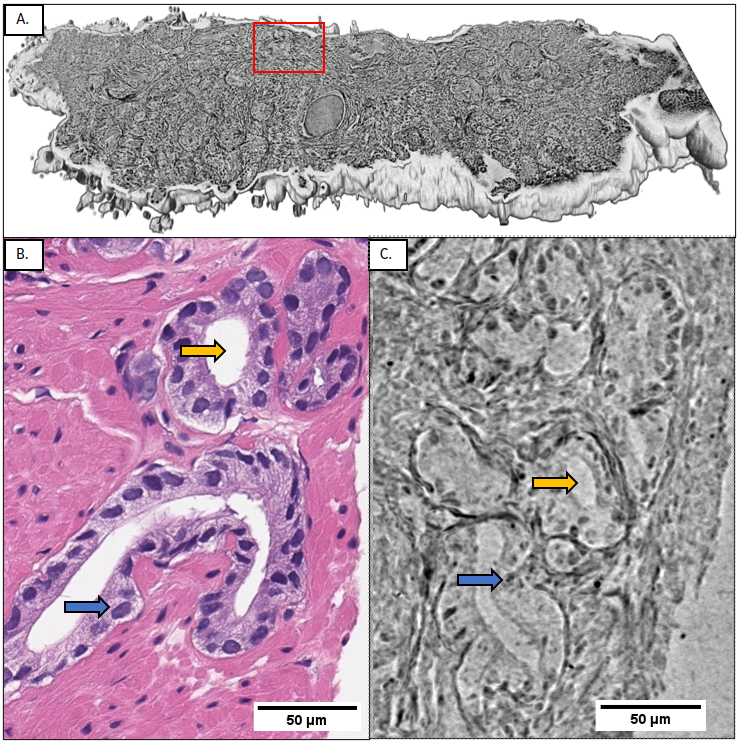
\includegraphics[width=0.69\textwidth]{ ./figures/figure1_v3.png }
  \caption{ PBCT imaging can resolve glandular structure in prostate biopsies.
    (A) 3D rendering of unstained FFPE prostate cancer scanned at LBNL, with a red box around the approximate region of panel C. (B) Histopathology slide taken from a malignant biopsy core, 20X
    magnification cropped to highlight a section of malignant glands. Nuclei
    (blue arrow) and lumen (orange arrow) are marked for comparison. (C) 5$\mu$m
    2D projection of a 3D image obtained from a PBCT scan of the same sample
    zoomed in to roughly the same region of malignant glands as shown in Panel
    B. Nuclei (blue arrow) are prominent. The lumina of glands (orange arrow)
    along with their borders are clearly defined. We obtained this PBCT image at
    the LBNL synchrotron at \(K=14keV\) and
    \(R=50mm\) without contrast-enhancing stain. The entire biopsy was
    imaged, only a small subset of that scan is included for
    brevity.}\label{fig:match_histo}
\end{wrapfigure}

PBCT experiments will take place at the ALS of LBNL, which will undergo maintenance later next year (2024). If we are unable to complete data collection prior to maintenance, Dr. Cheng maintains an active collaboration with the Advanced Photon Source (APS) of Argonne National Laboratory. We will conduct remaining imaging at the APS if necessary.

\subsection*{Aim 2: Evaluate utility of PBCT imaging for the grading of prostate cancer.}
Histopathology of prostate tissue biopsies is the gold standard for the diagnosis and grading of prostate cancer~\cite{epstein_prostate_2018}.
% NOTE Here is the one added sentence
% NOTE If you have space to add a figure, may want to reproduce (and cite) an open source image of Gleason score (something simple but illustrative). Not needed if no space.
Grading is based on the Gleason score~\cite{epstein_prostate_2018,ozkan_interobserver_2016,flach_significant_2021}, which typically ranges from 3 to 5 and is primarily defined by glandular morphology within the prostate.
% NOTE end added sentence
However, prior work has shown that Gleason scores can be highly variable both
between clinicians and even when the same clinician is shown different slices of
the same prostate biopsy~\cite{koyuncu_visual_2023}.% (is the later true)
This high variability can lead to either under- or over-treatment. It is
hypothesized that scoring based on 3D images may be superior to scoring based on
2D images. Unfortunately, directly testing this hypothesis confronts a form of
\textit{familiarity bias} since clinicians are trained on traditional slide-based
imaging. As a result, here we focus only on a proof of concept focused on
testing whether 3D imaging is non-inferior to 2D imaging. To test this
hypothesis we will collect, and make available, the first 3D imaging study of
prostate cancer.
%%% Are we actually going to show clinicians 3D images? maybe we go with neuro/glancer 3-panel images instead of MIPs and propose mips as the alternative strategy
%%%% It might be best to add a few words to clarify how gleason score is assigned

\subsubsection*{Develop 3D imaging study of prostate cancer.}
In collaboration with Dr. Warrick at PSU we will obtain whole-biopsy PBCT images of 20 age-matched benign and malignant prostate samples (see letter of reference). We will follow the same protocol used for generation of Figure 2B which already established that we can collect high-quality whole-biopsy images of similar biopsies provided by Dr. Warrick. For comparison, after imaging, each sample will be sliced and prepared for slide-based imaging using standard laboratory protocols. To make this data available as a public resource, both the slide-based images as well as the raw and 3D rendered PBCT images will be made available online using the same web-server developed in Aim 1.

\subsubsection*{Evaluate the hypothesis that 3D imaging can be used for scoring prostate cancer.}
In collaboration with Dr. Warrick (see letter of reference), the Chief of Clinical Pathology at Penn State College of Medicine (PSCOM), we will recruit up to 10 clinical pathologists (Fellows and Attendings) within and external to PSCOM to score 3D and 2D images of prostate biopsies. Each pathologist will be asked to provide Gleason scores for each of the prostate biopsies. For each biopsy a pathologist will be shown at random either the 3D rendering first or the 2D slide-based image first. After providing an initial score, they will then be shown the other imaging type and asked if they need to update their score based on the additional information provided by the second imaging modality. To avoid potential biases, we will randomize the order of samples for each pathologist and for each biopsy randomize whether pathologists are shown the 2D or 3D images first. Ultimately this will result in a two-by-two contingency table \(Y\) tabulating the number of individuals shown the 2D or 3D images first and whether or not they found the second imaging modality added information compared to the first.

We will test our hypothesis using standard tools from categorical data analysis. We will use a binomial test to evaluate the null hypothesis that the proportion of times where 3D imaging added information to 2D imaging (\(p_{1}\)) is greater than the proportion of times where 2D imaging added information to 3D imaging (\(p_{0}\)). To account for repeated measures we will formulate this test using binomial mixed effects models. To account for familiarity bias we will formulate this as a non-inferiority test with null hypothesis \(H_{0}:\log p_{1}/p_{0},\leq \delta\) where we will choose  \(\delta>0\) rather than \(\delta=0\) to provide a non-inferiority margin. We will chose \(\delta\) based on the results of a small pilot which will have a similar design to this one but 2D maximal intensity projections (MIPs) from 3D images will be shown rather than full 3D renderings. As in Figure 1, we will show the same region of biopsies using each imaging modality to ensure that the information content between the two imaging types is the same. Participants will be blinded to this fact and therefore we expect that we can estimate \(\delta=\log p_{1}/p_{0}\) using this pilot study. Note, our sample size is designed to achieve \(>85\%\) power under an alternative \(\log p_{1}/p_{0}\geq 0.2\) with a non-inferiority margin \(\delta\leq-0.2\).

\begin{wrapfigure}[24]{r}{0.5\textwidth}
  \vspace{-0.2cm} 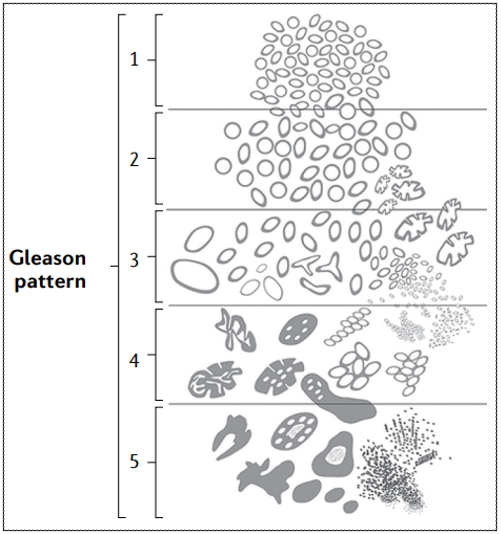
\includegraphics[width=0.49\textwidth]{ ./figures/ggrade1.png }
  \caption{Diagram of different patterns in glandular morphology and the associated Gleason grade. This figure was taken from a review by Rebello et. al~\cite{rebello_prostate_2021}.}\label{fig:setup}
\end{wrapfigure}

\subsubsection*{Potential Pitfalls and Alternative Strategies}
The major limitation we foresee is the complication of \textit{familiarity bias} wherein pathologists will be less likely to find PBCT useful solely because they are unfamiliar with the technology. If our preliminary study estimates \(\delta\geq 0.4\), we will compare gray-scale slide-based imaging to PBCT imaging. While standard slide based imaging is often colored, removing this color will likely mitigate the familiarity bias between these two imaging modalities while still allowing for meaningful comparisons.
%%% this is a great use of the idea to remove the color of histo slides

\subsection*{Aim 3: Quantify the morphological heterogeneity in prostate glands using computational persistent homology.}
The morphologic features of prostate glands that indicate cancer are abstract and difficult to quantify using standard statistical tools. For example, Figure 2 shows different glandular morphologies associated with different stages of cancer. The differences between Gleason pattern 5 (more diseased) and pattern 1 (healthy) are complex: it is not just a difference in size or volume but a difference of more abstract qualities like ``tortuousness''. It is not clear how to quantify these abstract morphologic features let alone how to incorporate some quantitative metric of this characteristic into models. Yet, there are numerous potential benefits from quantifying these characteristics. For example, if we could quantify Gleason patterns it would provide a more quantitative approach to staging cancer and might improve upon the current Gleason scoring system. Moreover, if we could quantify these characteristics then we could use those characteristics in statistical or machine learning models to help predict patient outcomes and guide treatment decisions. In this aim we borrow computational tools developed for macroscopic morphologic analysis of cancer and adapt those tools to the microscopic study of prostate cancer. We then demonstrate those tools by performing the first analysis of morphologic variation within prostate cancer.
% need a better figure for persistence diagram and filtration

\subsubsection*{Overview of Computational Persistent Homology}

Topology is a field of mathematics that, like geometry, studies shapes (See Wasserman et. al~\cite{wasserman_topological_2018} for a review on the distinction between these fields). Homology is a subfield of topology that specifically studies the voids or holes in shapes. In the context of prostate cancer, homology can be thought of as the natural field of mathematics for modeling glands which are essentially defined by their voids (i.e., lumen). In recent years, homology has moved from a field of abstract math to a powerful framework for modeling shapes thanks to advances in an area of applied statistics called computational persistent homology~\cite{wasserman_topological_2018,chazal_introduction_2021}. In brief, suppose that our shape is defined by a point cloud (e.g., a series 3D points each representing the nucleus of an epithelial cell of a gland). Next pretend that there is a ball of radius \(r\) centered about each point. Wherever two balls connect, create an edge between the corresponding points. This forms a graph. Rather than just forming one graph, create a series of graphs as \(r\) increases from 0 to infinity. In the language of computational persistent homology this is called a series of simplicial complexes (graphs) formed via a Rips filtration (formed by creating graphs as a function of \(r\)). The field of computational persistent homology has created a wide variety of statistics which summarize this series of simplicial complexes in such a way that the resulting statistics capture all the relevant information about homology (points, holes, voids) of the original shape. Those summary statistics can then be used in standard statistical and machine learning models.
%%% i should add info at the ''this forms a graph`` sentence on how this connects with persistence diagrams or barcode plots
%%% if persistence diagram, then have to include that in the figure and not just a barcode plot

\subsubsection*{Identify Morphologic Features Distinguishing Healthy and Cancerous Prostate Glands} \label{aim3.1}

In collaboration with Dr. Silverman, we will use 3D renderings of PBCT scans of prostate cancer developed in Aim 2 for the identification of morphologic features that distinguish healthy from cancerous prostate glands. Using those scans we will create a labeled dataset of over 100,000 images using standard synthetic-data techniques from computer vision: each rendering will be subset into 500 contiguous, randomly selected sub-regions; each sub-region will be randomly rotated, flipped, and inverted to create no fewer than 10 synthetic copies of the original sub-region; additional noise will be added to those synthetic copies to ensure robustness of learned morphologic features to measurement noise. Contrast-based thresholding of each image will be used to extract point clouds focused on gland cell nuclei. Each point-cloud will then be transformed via the Smooth Euler Characteristic Transform (SECT; which is a statistic calculated from a filtration over the point-cloud) that was recently introduced by Crawford et al.~(2020)~\cite{crawford_predicting_2020} for predicting patient outcomes in Glioblastoma Multiforme from morphologic features in MRI images. Importantly, the SECT maintains information about the homology of the point cloud but transforms that information into the space of smooth functions (into a Sobolev space). This is important as there are numerous statistical and machine learning tools available for modeling such smooth functions.
%%% reword first sentence
%%% contrast-based
%%% be more specific on''gland cell?`` probably not because you wont necessarily be able to prove exactly which cell type they are
%%% review cubic spline basis and sobolev space

\begin{wrapfigure}[7]{r}{0.6\textwidth}
  \vspace{-.3cm} 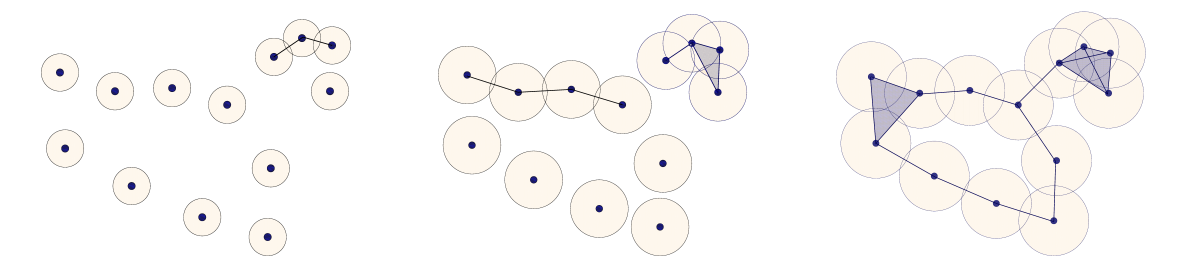
\includegraphics[width=0.59\textwidth]{ ./figures/vr.png }
  \caption{Illustration of a Vietoris-Rips complex being formed about a point cloud}\label{fig:setup}
\end{wrapfigure}

\textit{Using this function representation, we will turn the problem of identifying morphologic features into an equivalent problem of identifying a small number of simple functions that can distinguish whether an image came from a cancer or healthy biopsy.} More specifically, after turning each synthetic image into a continuous function, those functions will be decomposed into a cubic-spline basis. We will then use standard variable selection techniques from machine learning to identify a small number of components splines that are best able to classify the images. Such tools include penalized regression based methods (e.g., \(\ell_{1}\) penalized logistic regression) as well as algorithmic approaches (e.g., forward selection). Standard techniques such as cross validation will be used to help ensure the generalizability of identified morphologic features. Combined with our synthetic data techniques and our use of an age-matched cohort, this approach will ensure that the morphologic features we identify are robust. \emph{Ultimately this study will provide a set of morphological features that can be used to answer these questions directly in a low-dimensional (e.g., $<$5 dimensional) vector, providing a concise yet maximally informative representation of the critical morphological characteristics that distinguish healthy versus cancerous prostate tissue.}

\subsubsection*{Characterize Morphologic Variation in Prostate Glands} \label{aim3.2}
Is unknown whether the variation in the morphologic features distinguishing cancer is greater within a single prostate biopsy, between biopsies, or separately as a function of age. Answering such questions may provide fundamental insights into the heterogeneity of prostate cancer and are important considerations when designing clinical studies. Yet it has not been possible to directly answer these questions as we have lacked quantifiable morphologic features indicative of prostate cancer. In this aim, we use image features to perform the first quantitative analysis of morphologic variation in prostate glands and thereby answer such questions.
% check on the use of explicitly stating images

We will use the results of the prior subaim to calculate the morphological characteristics distinguishing healthy versus cancerous glandular structure. We will model the resulting data using multivariate mixed-effects models with variance components to identify the relative variation in morphologic structure within a biopsy, between biopsies of age- and disease-matched individuals, between biopsies taken over disease-matched biopsies taken from subjects of different ages, and between age-matched biopsies that differ in disease status. Spatial correlation between morphologic features will be accounted for using a first-order conditional-autoregressive variance component. \emph{Overall, this will result in a form of multivariate ANOVA where the relative contributions of different factors (e.g., space, age, disease status) to overall morphologic variation will be quantified.}
%%% here subaim is said but i have no explicit subaims - should i define one or is this common practice?

\subsubsection*{Potential Pitfalls and Alternative Approaches} \label{aim3-pitfalls}
Overall the modeling components of this aim are relatively straightforward as they make use of established statistical and machine learning tools that are commonly used within the Silverman lab. The major complication we might encounter is challenges in sampling glandular point-clouds from 3D rendered PBCT images. Based on our preliminary analyses of PBCT imaging of prostate biopsies (e.g., Figure 1), this does not seem likely. Still, it is possible that variation within disease phenotypes such as variation in stromal density or patterns of necrosis may complicate this task. Should we encounter this challenge, we will switch from simple contrast-based thresholding to newer deep-learning based image segmentation algorithms (e.g., Ilastik) which we have previously used to segment specific structures in micro-CT images~\cite{yakovlev_quantitative_2023}. Once segmented, point-clouds can be generated by uniformly sampling within the segmented gland regions.

\subsection*{Timeline}
% d the success of each aim helps to further subsequent aims
%
%        * When updating the research strategy make it explicitly clear at the end (given our preliminary data we are ready to begin work on EACh of these aims. They are independent but functionally synergistic)
\emph{Given our preliminary data, we are ready to begin the propsed work for each aim simultaneously. They are independent, but functionally synergistic.} The success of each aim is not dependent on previous aims. We have already optimized PBCT for imaging prostate biopsies and therefore Aim 2 can be performed without Aim 1. Similarly, we already have high-resolution full-biopsy images from a small number of healthy and cancerous prostate biopsies and therefore we can begin preliminary work on Aim 3 even before obtaining the full dataset proposed in Aim 2. Moreover, each aim will correspond to at least one first-author publication. The proposed aims will be distributed evenly across the years of this award. Preliminary data and current work (Y0) provide a foundation for the experiments of Aim 1 that will extend into year 1 of the award. Additional imaging time at LBNL in year 1 will allow data collection for Aim 2. In between imaging allocations we will recruit pathologists and perform a preliminary study. Upon completion of imaging experiments we will test the non-inferiority of our method. Aim 3 will begin with preliminary concept study and algorithm development independent of images and will result in a morphologic analysis of variation over years 1 and 2 of the award. In years 3 and 4 of the award (medical years denoted M) thesis and manuscript edits will be made during dedicated research blocks. Below we provide a timeline for completion of each major task.

\vspace{10pt}
\begin{minipage}{\textwidth}
  \begin{center}
    \begin{tabular}{|l|c|c|c|c|}
      \hline
      \textbf{Aims}                                        & \textbf{G3} & \textbf{G4} & \textbf{M3}  & \textbf{M4} \\
      \hline
      \textbf{A1:} Perform Imaging for PCBT Atlas  & \colcell     &      \colcell      &  &  \\
      \hline
      \textbf{A1:} Develop Neuroglancer Web Interface for Atlas  &   \colcell   &  \colcell             &  &    \\
      \hline
      \textbf{A2:} Perform PCBT Imaging for Prostate Cancer Study                         &            \colcell  &  \colcell    &  & \\
      \hline
      \textbf{A2:} Recruit and Survey Clinical Pathologists                          & & \colcell     &     &     \\
      \hline
      \textbf{A2:} Perform Data Analysis to Test Non-Inferiority &  & \colcell & \colcell & \\
      \hline
      \textbf{A3:} Perform Morphologic Analysis of Variation  &           & \colcell & \colcell  &    \\
      \hline
      \textbf{All:} Edit thesis and First-Author Manuscripts &             &  \colcell    & \colcell  &  \colcell  \\
      \hline
      \textbf{All:} Explore Translational Applications of Aims&        &       &  \colcell & \colcell \\
      \hline
    \end{tabular}
  \end{center}
\end{minipage}
\\[5pt]
% TODO Be consistent with we vs. We
\subsection*{Future Directions}
%mention the difficulty associated with large 3D datasets and cite xie paper
At the completion of this study, we will have developed the first protocol for high-resolution, stain-free, 3D imaging of whole soft-tissue biopsies and we will have evaluated the utility of this technology in the context of prostate-cancer. This work will open up multiple promising avenues for future research. We highlight just three. First, the PBCT imaging protocol we develop and demonstrate in Aim 1 is not limited to prostate cancer. Based on this technology, my approaches to prostate cancer in Aim 2 and 3 could be easily adapted to study other soft-tissue cancers. Second, Aim 2 only serves to evaluate the utility of PBCT imaging in the context of prostate cancer. Should Aim 2 establish that PBCT imaging can be used to grade prostate cancer, future work is needed to more formally study best practices for how to integrate PBCT imaging into clinical-practice. Finally, our analysis of morphologic variation is just one potential use for the morphologic features we develop in Aim 3.  Future studies will be needed to evaluate the utility of these features as biomarkers for diagnosis, prognosis, and treatment of disease.

\newpage
\bibliographystyle{nihunsrt}
\bibliography{sugarman_f30.bib}
\end{document}

% NOTE: JDS code for power analysis
% n <- 200
% S <- 10000
% p <- 0.45
% delta <- 0.1

% reject <- rep(NA, S)
% for (s in 1:S) {
%   y <- rbinom(n, 1, p)
%   fit <- binom.test(sum(y), n, p=driver::invLogit(0.2), alternative="less")
%   reject[s] <- fit$p.value
% }
% sum(reject<0.05)/S
% driver::Logit(p)
\begin{wrapfigure}[23]{r}{10cm}
  \vspace{-.6cm} 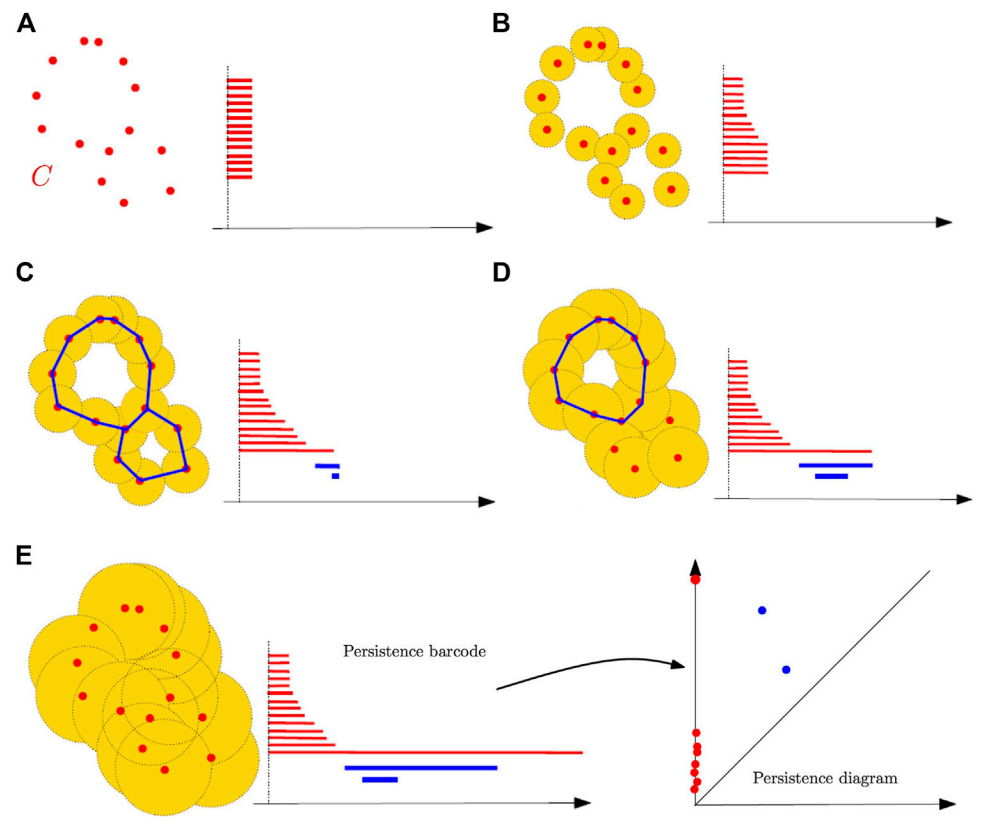
\includegraphics[width=10cm]{ ./figures/chazal_2.png }
  \caption{A.) Example point cloud sampled from a 3D shape and a barcode representing each point as an individual connected component. B.) The same point cloud with a rips filtration beginning. Some connected components persist and others merge with their neighbors at this stage of the filtration, leading to changes in the barcode plot. In (C) and (D) several components merge to form holes, recording an additional homology group in the barcode plot. Figure adapted from review by Chazal et. al~\cite{chazal_introduction_2021-1}.}\label{fig:setup}
\end{wrapfigure}

\begin{wrapfigure}[21]{r}{10cm}
  \vspace{-.6cm} 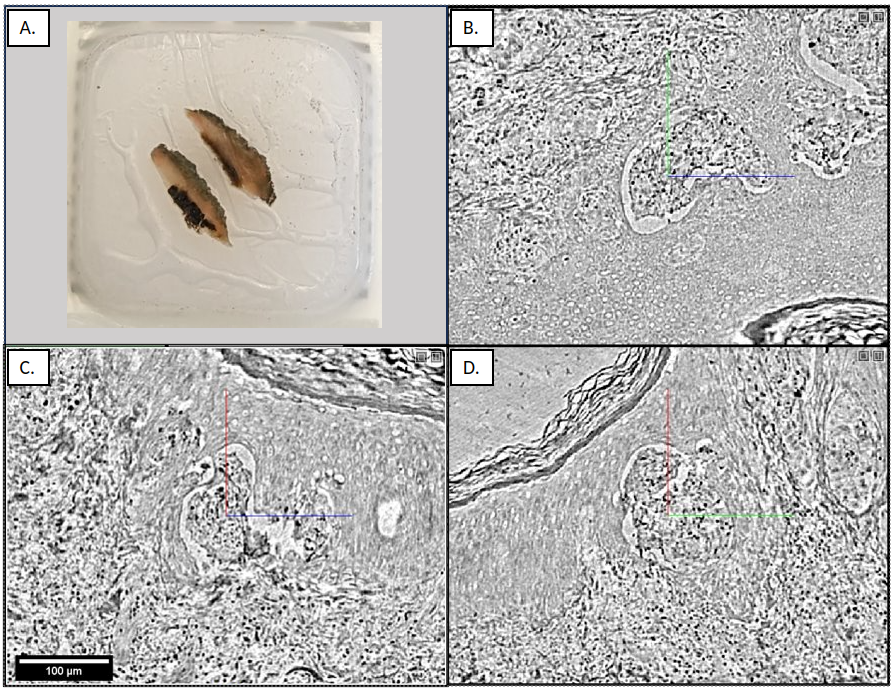
\includegraphics[width=10cm]{ ./figures/ngv1.png }
  \caption{A.) Tissue block containing unstained, FFPE, nodular melanoma. A, B, and C provide a 3-panel view of 1 FOV of a PBCT scan of an unstained FFPE melanoma biopsy (A) hosted on the Cheng Lab adaptation of the Neuroglancer web visualization tool~\cite{google_neuroglancer_2023}. With PBCT and Neuroglancer the user is able to adjust the window level of the image and scroll throughout the 3D volume at 0.5$\mu$m steps in each direction.}\label{fig:setup}
\end{wrapfigure}

\begin{wrapfigure}[31]{l}{0.6\textwidth}
  \vspace{-.5cm} 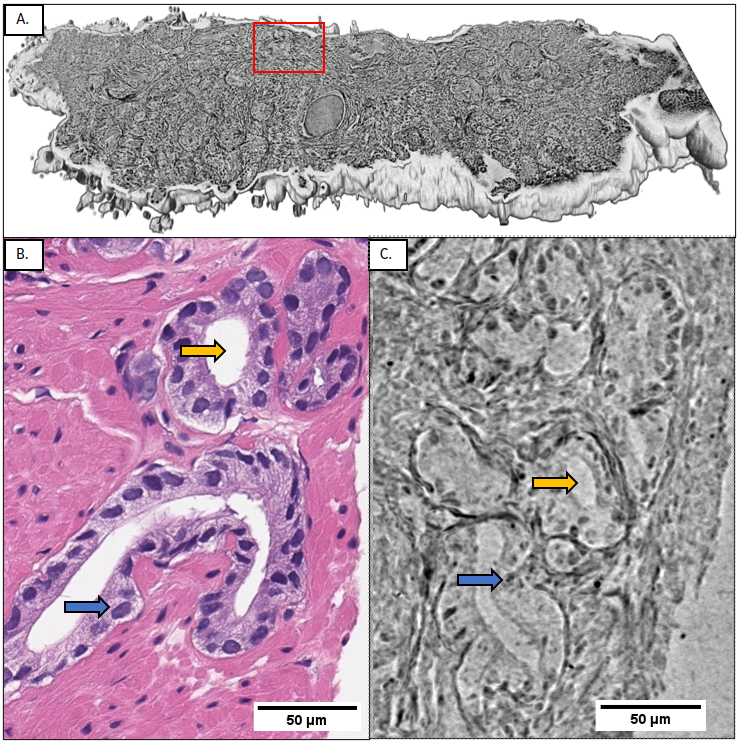
\includegraphics[width=0.59\textwidth]{ ./figures/figure1_v3.png }
  \caption{ PBCT imaging can resolve glandular structure in prostate biopsies.
    (A) 3D rendering of unstained FFPE prostate cancer scanned at LBNL, with a red box around the approximate region of panel C. (B) Histopathology slide taken from a malignant biopsy core, 20X
    magnification cropped to highlight a section of malignant glands. Nuclei
    (blue arrow) and lumen (orange arrow) are marked for comparison. (C) 5$\mu$m
    2D projection of a 3D image obtained from a PBCT scan of the same sample
    zoomed in to roughly the same region of malignant glands as shown in Panel
    B. Nuclei (blue arrow) are prominent. The lumina of glands (orange arrow)
    along with their borders are clearly defined. We obtained this PBCT image at
    the LBNL synchrotron at \(K=20keV\) and
    \(R=80mm\) without contrast-enhancing stain. The entire biopsy was
    imaged, only a small subset of that scan is included for
    brevity.}\label{fig:match_histo}
\end{wrapfigure}

\begin{wrapfigure}[31]{l}{0.6\textwidth}
  \vspace{-.5cm} 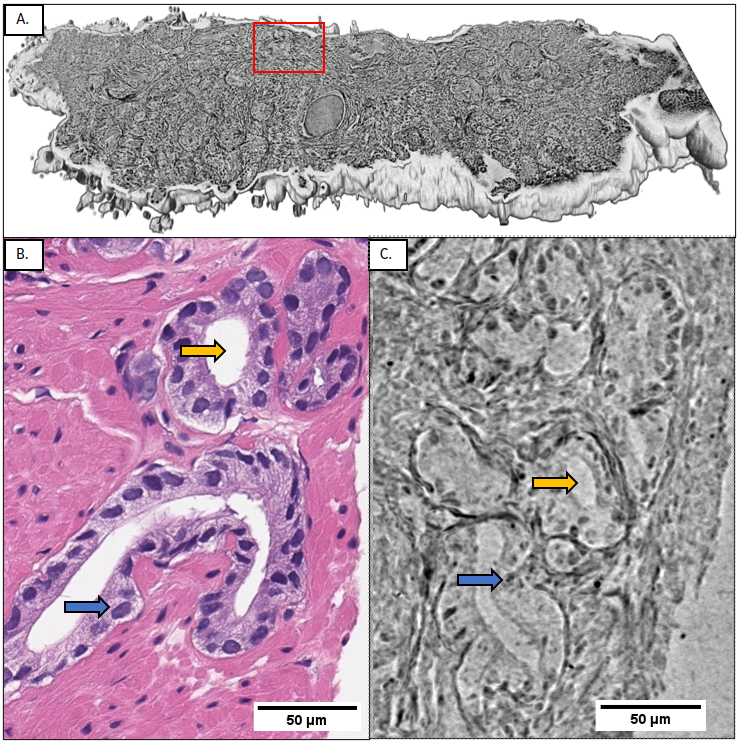
\includegraphics[width=0.59\textwidth]{ ./figures/figure1_v3.png }
  \caption{ PBCT imaging can resolve glandular structure in prostate biopsies.
    (A) 3D rendering of unstained FFPE prostate cancer scanned at LBNL, with a red box around the approximate region of panel C. (B) Histopathology slide taken from a malignant biopsy core, 20X
    magnification cropped to highlight a section of malignant glands. Nuclei
    (blue arrow) and lumen (orange arrow) are marked for comparison. (C) 5$\mu$m
    2D projection of a 3D image obtained from a PBCT scan of the same sample
    zoomed in to roughly the same region of malignant glands as shown in Panel
    B. Nuclei (blue arrow) are prominent. The lumina of glands (orange arrow)
    along with their borders are clearly defined. We obtained this PBCT image at
    the LBNL synchrotron at \(K=20keV\) and
    \(R=80mm\) without contrast-enhancing stain. The entire biopsy was
    imaged, only a small subset of that scan is included for
    brevity.}\label{fig:match_histo}
\end{wrapfigure}
